\subsection{Laboratory : Static Circuits}

In this fourth lab , we are going to use our knowledge of subthreshold transistors to characterize two circuits : the differential pair and the Bumb antibumb.

To measure small current (in our case from 1 pA to 10 nA) we are going to use a converter circuit, which will map current to frequency (C2F). Be aware of this because later on we need to map back our results to current. 

Today, you will also be first exposed to a Multiplexer and demultiplexer (mux/demux) circuit. The transistors we use are very tiny and numerous, but the input-output pins and C2F converters are unfortunately spacious. Therefore, we need mux/demux to select the circuits that we want at the beginning of each lab. 

Another functional circuit we use is the Bias Generator. It will make sure that all transistors work in the subthreshold regime by mirroring a current to the circuits that we need. 

Thus, we have three functional circuits that can let us advance to more complicated experiments . These are : 
- C2F converter
- Multiplexer and demultiplexer
- Bias Generator 

They are here to help you, just be aware of them. 

\subsubsection{N-FET differential pair circuit (NDP)}
\label{lab:diffpair}
First, we need to calibrate the C2F converter and the bias generator. To calibrate the output of C2F, we set a high voltage differential between $V_1$ and $V_2$ (i.e. around 0.4V) and we loop through a range of bias currents. We than read the output (which are frequencies) on the $I_1$ and $I_2$. This way we have a dictionary to refers to when we map frequency back to current in a later stage. 

The interesting part starts now. We fix a common voltage between $V_1$ and $V_2$ and we loop through a range of $V_1$ and $V_2$ that respect this common voltage constraint. 

$I_1$ becomes dominant when the differential $V_1-V_2$ is higher than -0.1V. The two output current are symmetrical, whereas the difference between the two is a sinusoidal. Overall, the current in the circuit is always equal to the bias current $I_b$.

\begin{figure}[H]
    \centering
    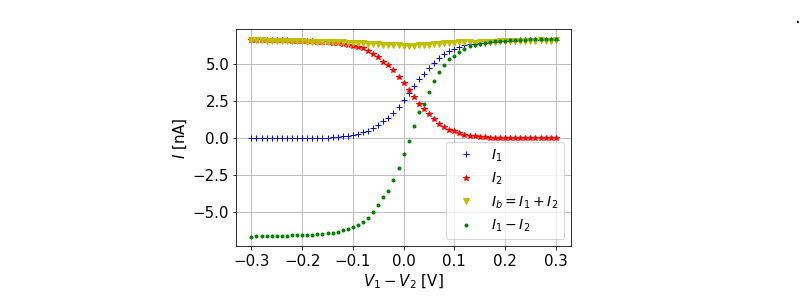
\includegraphics[width=0.95\linewidth]{Figures/diff_pair.png}
    \caption{Interpolated differential pair currents plotted over the voltage difference $V_1-V_2$}
    \label{fig:basalandcerebellum}
\end{figure}

If we increase the bias or the common mode, we can increase the current flowing in the circuit, hence, also the maximum ampere of $I_1$ and $I_2$. 

In the range of linearity, we observe that the offset voltage is slightly greater than zero because the two transistors are not exactly the same (as it is in theory assumed by the model). 
We note that the scale of the linearity range is the thermal voltage because the transistor is running under the weak inversion regime.
We speculated that if the regime was strong inversion, the overdrive would have determined this range, but it turned out we were wrong.  

\subsubsection{Bumb antibump}

The process to get results in the Bumb Anti Bumb circuit is comparable to the one used before \label{lab:diffpair}. We calibrate the channels and then we extract results varying $V_1$ and $V_2$ under a common voltage constraint (i.e. 0.9V). 

\begin{figure}[H]
    \centering
    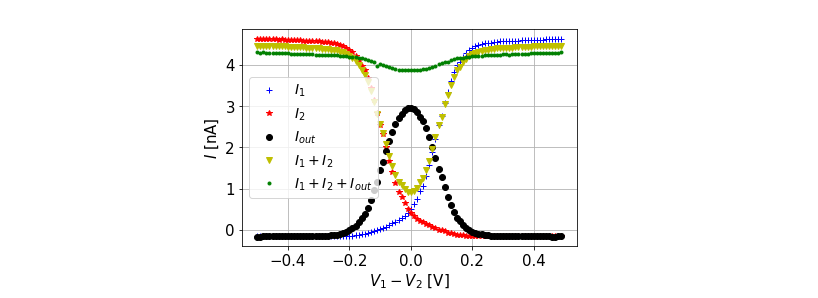
\includegraphics[width=0.95\linewidth]{Figures/antibumb.png}
    \caption{Interpolated Bumb AntiBumb plotted over the voltage difference $V_1-V_2$}
    \label{fig:basalandcerebellum}
\end{figure}

What is important to notice, is that the sigma of the Guassian distribution $I_{out}$ (sorry for the approximation, but I see Bell curves everywhere) it's proportional to the current $I_b$. Keep this in mind, but don't bring it up near to Tobi because it awakens bad memories to him ;).  

The behavior of $I_{out}$ is very well defined because we are interpolating frequencies outputs. Therefore, we can easily fit a quadratic function to the sum $I_1+I_2$ and a linear function for the individual components.

\begin{figure}[H]
    \centering
    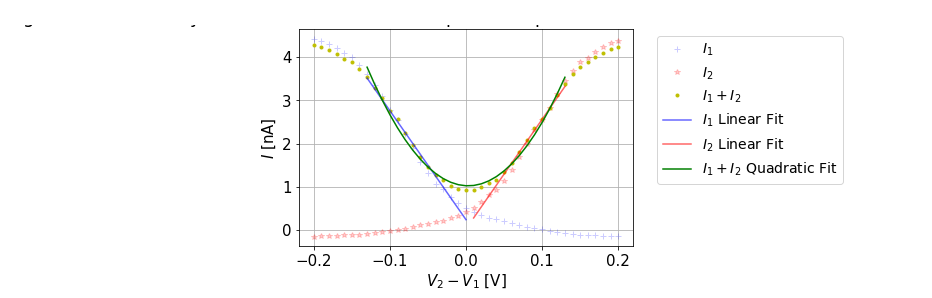
\includegraphics[width=0.95\linewidth]{Figures/antibumb_approx.png}
    \caption{Quadratically fitted interpolated Bumb AntiBumb plotted over the voltage difference $V_1-V_2$}
    \label{fig:basalandcerebellum}
\end{figure}



